\documentclass[
	letterpaper, % Paper size, specify a4paper (A4) or letterpaper (US letter)
	10pt, % Default font size, specify 10pt, 11pt or 12pt
]{CSUniSchoolLabReport}

\DeclareSIUnit \siemen {S}

%----------------------------------------------------------------------------------------
%	REPORT INFORMATION
%----------------------------------------------------------------------------------------

\title{Homework 8/9\\ Fundamentals of Electronics \\ EECE2412/3} % Report title

\author{Michael \textsc{Brodskiy}\\ \small \href{mailto:Brodskiy.M@Northeastern.edu}{Brodskiy.M@Northeastern.edu}}

\date{November 21, 2024} % Date of the report

%----------------------------------------------------------------------------------------


\begin{document}

\maketitle % Insert the title, author and date using the information specified above

\begin{center}
	\begin{tabular}{l r}
		Instructor: & Professor \textsc{Onabajo} \\ % Instructor/supervisor
	\end{tabular}
\end{center}

\newpage

\begin{abstract}

  The purpose of this document is to outline the design process for a common-emitter bipolar junction transistor (BJT) amplifier with specified characteristics. The design process involved creating a viable circuit, calculating expected results, and simulating to confirm expectations.

\end{abstract}

\begin{flushleft}

  \textsc{Keywords:} \underline{common-emitter}, \underline{BJT}, \underline{amplifier} 

\end{flushleft}

\newpage

\tableofcontents
\listoffigures

\newpage

\section{Introduction}

Common-emitter amplifiers are some of the most ubiquitous components of radio-frequency (RF) circuitry. These components, which rely on bipolar junction transistors (BJTs) involve the amplification of a source signal, passed through the base of the BJT. The base is connected to the collector branch via a resistor. To improve stability of such circuits, capacitors are added after the input and before the output, which allows for better direct-current (DC) filtration. Such amplification is crucial in audio-based circuits, like speakers, and radios, specifically antennas.

\section{Circuit Design}

We may begin with our provided model:

\begin{figure}[H]
  \centering
  \tikzset{every picture/.style={line width=0.75pt}} %set default line width to 0.75pt        

\begin{tikzpicture}[x=0.75pt,y=0.75pt,yscale=-1,xscale=1]
%uncomment if require: \path (0,445); %set diagram left start at 0, and has height of 445

%Straight Lines [id:da3205833586611301] 
\draw    (75,256.29) -- (75,302) ;
%Straight Lines [id:da9669601447516369] 
\draw    (196.43,256.29) -- (154,256.29) ;
%Straight Lines [id:da5342877285157912] 
\draw    (295.42,397.71) -- (154,397.71) ;
%Shape: Circle [id:dp43569553605319233] 
\draw   (50,327) .. controls (50,313.19) and (61.19,302) .. (75,302) .. controls (88.81,302) and (100,313.19) .. (100,327) .. controls (100,340.81) and (88.81,352) .. (75,352) .. controls (61.19,352) and (50,340.81) .. (50,327) -- cycle ;
%Straight Lines [id:da5510373866627751] 
\draw    (75,352) -- (75,397.71) ;
%Curve Lines [id:da30203956207151417] 
\draw    (50,327) .. controls (75,301) and (75,353) .. (100,327) ;
%Straight Lines [id:da21541767169381376] 
\draw    (295.42,256.29) -- (252.99,256.29) ;
%Shape: Contact [id:dp8866163118049385] 
\draw   (196.43,256.29) -- (213.4,256.29) (252.99,256.29) -- (236.02,256.29) (213.4,235.79) -- (213.4,276.79) (236.02,235.79) -- (236.02,276.79) ;
%Shape: Resistor [id:dp576364330099814] 
\draw   (295.42,176.29) -- (295.42,190.69) -- (315.42,193.89) -- (275.42,200.29) -- (315.42,206.69) -- (275.42,213.09) -- (315.42,219.49) -- (275.42,225.89) -- (315.42,232.29) -- (275.42,238.69) -- (295.42,241.89) -- (295.42,256.29) ;
%Straight Lines [id:da8771969312931523] 
\draw    (295.42,176.29) -- (337.85,176.29) ;
%Straight Lines [id:da41124917033766106] 
\draw    (337.85,176.29) -- (380.27,176.29) ;
%Shape: Resistor [id:dp32430912394809286] 
\draw   (380.27,91.44) -- (380.27,105.84) -- (400.27,109.04) -- (360.27,115.44) -- (400.27,121.84) -- (360.27,128.24) -- (400.27,134.64) -- (360.27,141.04) -- (400.27,147.44) -- (360.27,153.84) -- (380.27,157.04) -- (380.27,171.44) ;
%Straight Lines [id:da679079796492945] 
\draw    (422.7,171.44) -- (380.27,171.44) ;
%Shape: Contact [id:dp06576563479218167] 
\draw   (422.7,171.44) -- (439.67,171.44) (479.27,171.44) -- (462.3,171.44) (439.67,150.94) -- (439.67,191.94) (462.3,150.94) -- (462.3,191.94) ;
%Straight Lines [id:da0315404774607444] 
\draw    (521.7,171.44) -- (479.27,171.44) ;
%Straight Lines [id:da16395222634879947] 
\draw    (366.7,256.01) -- (295.42,256.29) ;
%Shape: Circle [id:dp09876127689341485] 
\draw   (347.7,256.01) .. controls (347.7,238.02) and (362.28,223.44) .. (380.27,223.44) .. controls (398.27,223.44) and (412.85,238.02) .. (412.85,256.01) .. controls (412.85,274) and (398.27,288.59) .. (380.27,288.59) .. controls (362.28,288.59) and (347.7,274) .. (347.7,256.01) -- cycle ;
%Straight Lines [id:da7855487082641662] 
\draw [line width=1.5]    (366.7,277.23) -- (366.7,234.8) ;
%Straight Lines [id:da6420856407737783] 
\draw    (380.27,223.86) -- (380.27,171.44) ;
%Straight Lines [id:da9346216852859565] 
\draw [line width=1.5]    (366.7,256.01) -- (379.12,285.82) ;
\draw [shift={(380.27,288.59)}, rotate = 247.38] [color={rgb, 255:red, 0; green, 0; blue, 0 }  ][line width=1.5]    (14.21,-4.28) .. controls (9.04,-1.82) and (4.3,-0.39) .. (0,0) .. controls (4.3,0.39) and (9.04,1.82) .. (14.21,4.28)   ;
%Straight Lines [id:da5297912314249998] 
\draw    (381,398) -- (380.27,376.59) ;
%Straight Lines [id:da006223218346351644] 
\draw [line width=1.5]    (366.7,256.01) -- (380.27,223.86) ;
%Straight Lines [id:da4306693520228567] 
\draw    (450.84,397.71) -- (295.42,397.71) ;
%Straight Lines [id:da9701929454236062] 
\draw    (380.27,376.59) -- (380.27,288.59) ;
%Straight Lines [id:da13224312413179473] 
\draw    (295.42,397.71) -- (295.42,414.13) ;
%Straight Lines [id:da10473520328776764] 
\draw    (311.84,418.13) -- (295.42,418.13) ;
%Straight Lines [id:da46427341450112913] 
\draw    (295.42,418.13) -- (279,418.13) ;
%Straight Lines [id:da9976365744338328] 
\draw    (303.42,426.13) -- (287,426.13) ;
%Straight Lines [id:da39363951353981896] 
\draw    (295.42,422.13) -- (283,422.13) ;
%Straight Lines [id:da2887972782852376] 
\draw    (307.84,422.13) -- (295.42,422.13) ;
%Straight Lines [id:da30358936692439087] 
\draw [line width=1.5]    (380.27,91.44) -- (380.27,39.02) ;
\draw [shift={(380.27,36.02)}, rotate = 90] [color={rgb, 255:red, 0; green, 0; blue, 0 }  ][line width=1.5]    (14.21,-4.28) .. controls (9.04,-1.82) and (4.3,-0.39) .. (0,0) .. controls (4.3,0.39) and (9.04,1.82) .. (14.21,4.28)   ;
%Shape: Resistor [id:dp4461598607548093] 
\draw   (74,256.29) -- (88.4,256.29) -- (91.6,236.29) -- (98,276.29) -- (104.4,236.29) -- (110.8,276.29) -- (117.2,236.29) -- (123.6,276.29) -- (130,236.29) -- (136.4,276.29) -- (139.6,256.29) -- (154,256.29) ;
%Straight Lines [id:da2766899928458427] 
\draw    (154,397.71) -- (75,397.71) ;
%Shape: Resistor [id:dp802419533777393] 
\draw   (521.7,242.44) -- (521.7,256.84) -- (541.7,260.04) -- (501.7,266.44) -- (541.7,272.84) -- (501.7,279.24) -- (541.7,285.64) -- (501.7,292.04) -- (541.7,298.44) -- (501.7,304.84) -- (521.7,308.04) -- (521.7,322.44) ;
%Straight Lines [id:da14948589225876163] 
\draw    (521.7,396.86) -- (450.84,397.71) ;
%Straight Lines [id:da47456571549507187] 
\draw    (521.7,396.86) -- (521.7,322.44) ;
%Straight Lines [id:da5473358720735196] 
\draw    (521.7,242.44) -- (521.7,171.44) ;
%Straight Lines [id:da27562690626686936] 
\draw    (561.77,171.44) -- (521.7,171.44) ;
\draw [shift={(564.12,171.44)}, rotate = 180] [color={rgb, 255:red, 0; green, 0; blue, 0 }  ][line width=0.75]      (0, 0) circle [x radius= 3.35, y radius= 3.35]   ;

% Text Node
\draw (102,330.4) node [anchor=north west][inner sep=0.75pt]    {$V_{S}$};
% Text Node
\draw (215.4,280.19) node [anchor=north west][inner sep=0.75pt]    {$C_{in} =200\left[ \Micro \text{F}\right]$};
% Text Node
\draw (317.42,210.09) node [anchor=north west][inner sep=0.75pt]    {$R_{B}$};
% Text Node
\draw (402.27,125.24) node [anchor=north west][inner sep=0.75pt]    {$R_{C}$};
% Text Node
\draw (462.3,195.34) node [anchor=north] [inner sep=0.75pt]    {$C_{out} =200\left[ \Micro \text{F}\right]$};
% Text Node
\draw (380.27,32.62) node [anchor=south] [inner sep=0.75pt]    {$+12\left[\text{V}\right]$};
% Text Node
\draw (100,279.69) node [anchor=north west][inner sep=0.75pt]    {$R_{S} =500[ \si{\ohm}]$};
% Text Node
\draw (543.7,276.24) node [anchor=north west][inner sep=0.75pt]    {$R_{L} =15\left[\text{k} \si{\ohm}\right]$};
% Text Node
\draw (566.12,174.84) node [anchor=north west][inner sep=0.75pt]    {$V_{out}$};
% Text Node
\draw (414.85,259.41) node [anchor=north west][inner sep=0.75pt]    {$Q_{1}$};


\end{tikzpicture}

  \caption{Standard Common-Emitter Amplifier}
  \label{fig:1}
\end{figure}

This, in tandem with the provided circuit example, will be the basis for our design.

\subsection{Given Parameters}

We are given the following parameters as a requirement for our amplifier:

$$\boxed{\left\{\begin{array}{ll}\text{Assume: }&T=300[\si{\kelvin}]\\|A_{VS}|=\frac{V_o}{V_{in}}&\geq 80\\I_C&\leq 8[\si{\milli\ampere}]\\V_{CC}&= 12[\si{\volt}]\\R_S&= 500[\si{\ohm}]\\R_L&= 15[\si{\kilo\ohm}]\\R_i&\approx R_S\\V_{FB}&=.7[\si{\volt}]\\\beta&=200\end{array}}$$

  Finally, we want to ensure that there is a $7[\si{\volt}]$ peak-to-peak output signal swing without distortion. We begin by performing a DC analysis of the given circuit.

\subsection{DC Analysis}

The DC equivalent circuit may be constructing by taking all capacitors as open circuits. This gives us an equivalent circuit of:

\begin{figure}[H]
  \centering
  \tikzset{every picture/.style={line width=0.75pt}} %set default line width to 0.75pt        

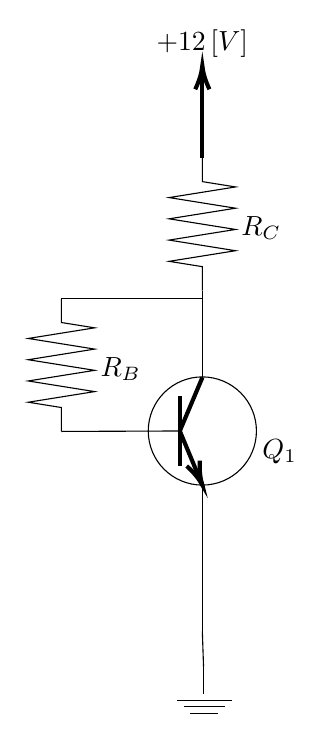
\begin{tikzpicture}[x=0.75pt,y=0.75pt,yscale=-.8,xscale=.8]
%uncomment if require: \path (0,445); %set diagram left start at 0, and has height of 445

%Shape: Resistor [id:dp576364330099814] 
\draw   (295.42,176.29) -- (295.42,190.69) -- (315.42,193.89) -- (275.42,200.29) -- (315.42,206.69) -- (275.42,213.09) -- (315.42,219.49) -- (275.42,225.89) -- (315.42,232.29) -- (275.42,238.69) -- (295.42,241.89) -- (295.42,256.29) ;
%Straight Lines [id:da8771969312931523] 
\draw    (295.42,176.29) -- (337.85,176.29) ;
%Straight Lines [id:da41124917033766106] 
\draw    (337.85,176.29) -- (380.27,176.29) ;
%Shape: Resistor [id:dp32430912394809286] 
\draw   (380.27,91.44) -- (380.27,105.84) -- (400.27,109.04) -- (360.27,115.44) -- (400.27,121.84) -- (360.27,128.24) -- (400.27,134.64) -- (360.27,141.04) -- (400.27,147.44) -- (360.27,153.84) -- (380.27,157.04) -- (380.27,171.44) ;
%Straight Lines [id:da16395222634879947] 
\draw    (366.7,256.01) -- (295.42,256.29) ;
%Shape: Circle [id:dp09876127689341485] 
\draw   (347.7,256.01) .. controls (347.7,238.02) and (362.28,223.44) .. (380.27,223.44) .. controls (398.27,223.44) and (412.85,238.02) .. (412.85,256.01) .. controls (412.85,274) and (398.27,288.59) .. (380.27,288.59) .. controls (362.28,288.59) and (347.7,274) .. (347.7,256.01) -- cycle ;
%Straight Lines [id:da7855487082641662] 
\draw [line width=1.5]    (366.7,277.23) -- (366.7,234.8) ;
%Straight Lines [id:da6420856407737783] 
\draw    (380.27,223.86) -- (380.27,171.44) ;
%Straight Lines [id:da9346216852859565] 
\draw [line width=1.5]    (366.7,256.01) -- (379.12,285.82) ;
\draw [shift={(380.27,288.59)}, rotate = 247.38] [color={rgb, 255:red, 0; green, 0; blue, 0 }  ][line width=1.5]    (14.21,-4.28) .. controls (9.04,-1.82) and (4.3,-0.39) .. (0,0) .. controls (4.3,0.39) and (9.04,1.82) .. (14.21,4.28)   ;
%Straight Lines [id:da5297912314249998] 
\draw    (381,398) -- (380.27,376.59) ;
%Straight Lines [id:da006223218346351644] 
\draw [line width=1.5]    (366.7,256.01) -- (380.27,223.86) ;
%Straight Lines [id:da9701929454236062] 
\draw    (380.27,376.59) -- (380.27,288.59) ;
%Straight Lines [id:da13224312413179473] 
\draw    (381,398) -- (381,414.42) ;
%Straight Lines [id:da10473520328776764] 
\draw    (397.84,418.13) -- (381.42,418.13) ;
%Straight Lines [id:da46427341450112913] 
\draw    (381.42,418.13) -- (365,418.13) ;
%Straight Lines [id:da9976365744338328] 
\draw    (389.42,426.13) -- (373,426.13) ;
%Straight Lines [id:da39363951353981896] 
\draw    (381.42,422.13) -- (369,422.13) ;
%Straight Lines [id:da2887972782852376] 
\draw    (393.84,422.13) -- (381.42,422.13) ;
%Straight Lines [id:da30358936692439087] 
\draw [line width=1.5]    (380.27,91.44) -- (380.27,39.02) ;
\draw [shift={(380.27,36.02)}, rotate = 90] [color={rgb, 255:red, 0; green, 0; blue, 0 }  ][line width=1.5]    (14.21,-4.28) .. controls (9.04,-1.82) and (4.3,-0.39) .. (0,0) .. controls (4.3,0.39) and (9.04,1.82) .. (14.21,4.28)   ;

% Text Node
\draw (317.42,210.09) node [anchor=north west][inner sep=0.75pt]    {$R_{B}$};
% Text Node
\draw (402.27,125.24) node [anchor=north west][inner sep=0.75pt]    {$R_{C}$};
% Text Node
\draw (380.27,32.62) node [anchor=south] [inner sep=0.75pt]    {$+12\left[\text{V}\right]$};
% Text Node
\draw (414.85,259.41) node [anchor=north west][inner sep=0.75pt]    {$Q_{1}$};


\end{tikzpicture}

  \caption{DC Equivalent Circuit}
  \label{fig:2}
\end{figure}

From this, we may use Kirchoff's voltage laws to write:

$$\boxed{12-(I_B+I_C)R_C-R_BI_B-V_{BE}=0}$$

We know $\beta$, which allows us to say:

$$200=\frac{I_C}{I_B}$$
$$I_C=200I_B$$

Substituting this into the above, we get:

$$12-I_B(201R_C+R_B)-.7=0$$

\subsubsection{Worst-Case Assumption}

Since $I_C\leq 8[\si{\milli\ampere}]$, we know that:

$$I_B\leq \frac{I_C}{200}$$
$$I_B\leq 40[\si{\micro\ampere}]$$

\subsubsection{Finding Applicable $R_B$ and $R_C$ Values}

Assuming worst-case (\textit{i}.\textit{e}. highest) values of the currents, we get $I_C=8[\si{\milli\ampere}]$ and $I_B=40[\si{\micro\ampere}]$. Plugging this in, we get:

$$11.3=(40\cdot10^{-6})(201R_C+R_B)$$
$$282500=201R_C+R_B$$
$$\boxed{R_C=\frac{282500-R_B}{201}}$$

We need $R_B$ to be positive, which means $201R_C<282500$. Let us take $R_C$ as an arbitrary $\boxed{R_C=.9[\si{\kilo\ohm}]}$, which gives us:

$$\boxed{R_B=101.6[\si{\kilo\ohm}]}$$

\subsection{Small-Signal Analysis}

We may redraw the circuit using the Hybrid-$\pi$ Model to obtain the small-signal equivalent:

\begin{figure}[H]
  \centering
  \tikzset{every picture/.style={line width=0.75pt}} %set default line width to 0.75pt        

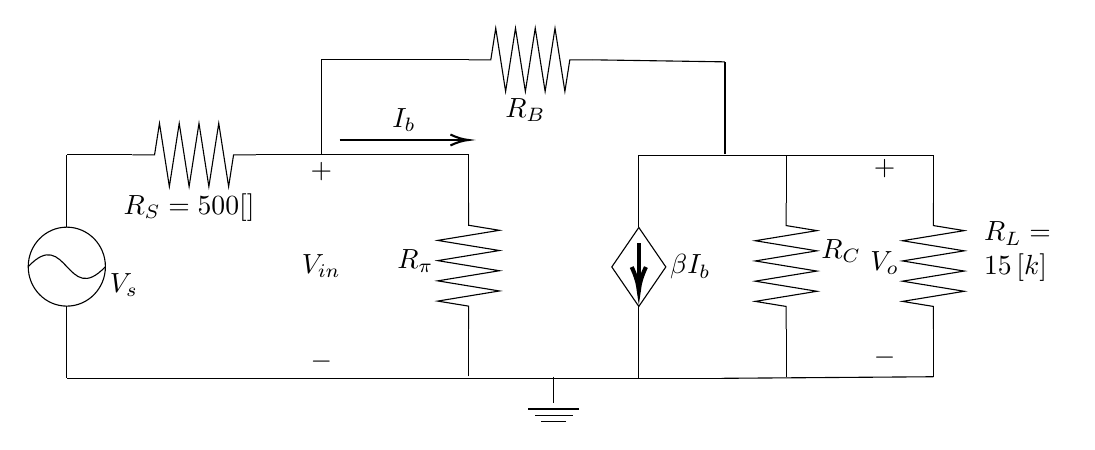
\begin{tikzpicture}[x=0.75pt,y=0.75pt,yscale=-.8,xscale=.8]
%uncomment if require: \path (0,445); %set diagram left start at 0, and has height of 445

%Straight Lines [id:da3205833586611301] 
\draw    (26.24,231.38) -- (26.24,274.87) ;
%Straight Lines [id:da9669601447516369] 
\draw    (65.68,231.38) -- (26.24,231.38) ;
%Straight Lines [id:da5342877285157912] 
\draw    (157.7,365.91) -- (26.24,365.91) ;
%Shape: Ellipse [id:dp43569553605319233] 
\draw   (3,298.65) .. controls (3,285.51) and (13.4,274.87) .. (26.24,274.87) .. controls (39.07,274.87) and (49.48,285.51) .. (49.48,298.65) .. controls (49.48,311.78) and (39.07,322.43) .. (26.24,322.43) .. controls (13.4,322.43) and (3,311.78) .. (3,298.65) -- cycle ;
%Straight Lines [id:da5510373866627751] 
\draw    (26.24,322.43) -- (26.24,365.91) ;
%Curve Lines [id:da30203956207151417] 
\draw    (3,298.65) .. controls (26.24,273.91) and (26.24,323.38) .. (49.48,298.65) ;
%Shape: Resistor [id:dp2331410449843161] 
\draw   (65.68,231.38) -- (79.07,231.38) -- (82.04,212.36) -- (87.99,250.41) -- (93.94,212.36) -- (99.89,250.41) -- (105.84,212.36) -- (111.79,250.41) -- (117.74,212.36) -- (123.69,250.41) -- (126.66,231.38) -- (140.05,231.38) ;
%Straight Lines [id:da13224312413179473] 
\draw    (319.45,364.96) -- (319.45,380.58) ;
%Straight Lines [id:da10473520328776764] 
\draw    (334.72,384.39) -- (319.45,384.39) ;
%Straight Lines [id:da46427341450112913] 
\draw    (319.45,384.39) -- (304.19,384.39) ;
%Straight Lines [id:da9976365744338328] 
\draw    (326.89,392) -- (311.63,392) ;
%Straight Lines [id:da39363951353981896] 
\draw    (319.45,388.19) -- (307.91,388.19) ;
%Straight Lines [id:da2887972782852376] 
\draw    (331,388.19) -- (319.45,388.19) ;
%Straight Lines [id:da9294247909853637] 
\draw    (179.49,202.74) -- (179.49,174.09) ;
%Straight Lines [id:da6388694575436823] 
\draw    (179.49,231.38) -- (140.05,231.38) ;
%Straight Lines [id:da16440166034456305] 
\draw    (179.49,231.38) -- (179.49,202.74) ;
%Shape: Resistor [id:dp48711677914528007] 
\draw   (268.19,174.09) -- (281.58,174.09) -- (284.55,155.07) -- (290.5,193.12) -- (296.45,155.07) -- (302.4,193.12) -- (308.35,155.07) -- (314.3,193.12) -- (320.25,155.07) -- (326.2,193.12) -- (329.17,174.09) -- (342.56,174.09) ;
%Straight Lines [id:da84456559815691] 
\draw    (422.61,230.89) -- (422.61,175.32) ;
%Straight Lines [id:da4153262290600702] 
\draw    (268.19,231.38) -- (179.49,231.38) ;
%Straight Lines [id:da343953647372656] 
\draw    (289.17,365.91) -- (157.7,365.91) ;
%Straight Lines [id:da9638367963246735] 
\draw    (420.63,365.91) -- (289.17,365.91) ;
%Straight Lines [id:da14254872853695066] 
\draw    (548.13,364.96) -- (420.63,365.91) ;
%Straight Lines [id:da6430168807157549] 
\draw    (268.19,260.03) -- (268.19,231.38) ;
%Shape: Resistor [id:dp13995844780538003] 
\draw   (268.19,260.03) -- (268.19,273.72) -- (286.78,276.77) -- (249.6,282.86) -- (286.78,288.94) -- (249.6,295.03) -- (286.78,301.12) -- (249.6,307.21) -- (286.78,313.3) -- (249.6,319.39) -- (268.19,322.43) -- (268.19,336.13) ;
%Straight Lines [id:da6369139211090866] 
\draw    (268.19,364.77) -- (268.19,336.13) ;
%Straight Lines [id:da1749405919965089] 
\draw    (370.72,322.62) -- (370.72,366.1) ;
%Flowchart: Decision [id:dp002686864136698386] 
\draw   (370.72,275.06) -- (386.99,298.84) -- (370.72,322.62) -- (354.45,298.84) -- cycle ;
%Straight Lines [id:da11250142173933209] 
\draw [line width=1.5]    (370.72,284.57) -- (370.72,310.11) ;
\draw [shift={(370.72,313.11)}, rotate = 270] [color={rgb, 255:red, 0; green, 0; blue, 0 }  ][line width=1.5]    (14.21,-4.28) .. controls (9.04,-1.82) and (4.3,-0.39) .. (0,0) .. controls (4.3,0.39) and (9.04,1.82) .. (14.21,4.28)   ;
%Straight Lines [id:da9690674503004082] 
\draw    (370.72,231.57) -- (370.72,275.06) ;
%Straight Lines [id:da5784113448919789] 
\draw    (459.42,231.57) -- (370.72,231.57) ;
%Shape: Resistor [id:dp5663551210845172] 
\draw   (459.42,260.22) -- (459.42,273.91) -- (478.01,276.96) -- (440.83,283.05) -- (478.01,289.14) -- (440.83,295.22) -- (478.01,301.31) -- (440.83,307.4) -- (478.01,313.49) -- (440.83,319.58) -- (459.42,322.62) -- (459.42,336.32) ;
%Straight Lines [id:da23800624757606248] 
\draw    (459.42,260.22) -- (459.42,231.57) ;
%Straight Lines [id:da16941854157492575] 
\draw    (459.42,364.96) -- (459.42,336.32) ;
%Straight Lines [id:da7883655281245964] 
\draw    (548.13,231.57) -- (459.42,231.57) ;
%Straight Lines [id:da5152336829111076] 
\draw    (268.19,174.09) -- (179.49,174.09) ;
%Straight Lines [id:da8468571314022476] 
\draw    (422.61,175.32) -- (342.56,174.09) ;
%Shape: Resistor [id:dp9552110757626432] 
\draw   (548.13,260.22) -- (548.13,273.91) -- (566.72,276.96) -- (529.53,283.05) -- (566.72,289.14) -- (529.53,295.22) -- (566.72,301.31) -- (529.53,307.4) -- (566.72,313.49) -- (529.53,319.58) -- (548.13,322.62) -- (548.13,336.32) ;
%Straight Lines [id:da33209874815771967] 
\draw    (548.13,260.22) -- (548.13,231.57) ;
%Straight Lines [id:da33021316124906264] 
\draw    (548.13,364.96) -- (548.13,336.32) ;
%Straight Lines [id:da42070751064178047] 
\draw    (190.49,222.38) -- (266.19,222.38) ;
\draw [shift={(268.19,222.38)}, rotate = 180] [color={rgb, 255:red, 0; green, 0; blue, 0 }  ][line width=0.75]    (10.93,-3.29) .. controls (6.95,-1.4) and (3.31,-0.3) .. (0,0) .. controls (3.31,0.3) and (6.95,1.4) .. (10.93,3.29)   ;

% Text Node
\draw (50.63,301.46) node [anchor=north west][inner sep=0.75pt]    {$V_{s}$};
% Text Node
\draw (99.89,253.22) node [anchor=north] [inner sep=0.75pt]    {$R_{S} =500[ \si{\ohm}]$};
% Text Node
\draw (248.55,295.03) node [anchor=east] [inner sep=0.75pt]    {$R_{\pi }$};
% Text Node
\draw (179.49,234.25) node [anchor=north] [inner sep=0.75pt]    {$+$};
% Text Node
\draw (179.49,298.5) node    {$V_{in}$};
% Text Node
\draw (179.49,362.75) node [anchor=south] [inner sep=0.75pt]    {$-$};
% Text Node
\draw (388.04,298.84) node [anchor=west] [inner sep=0.75pt]    {$\beta I_{b}$};
% Text Node
\draw (479.06,289.14) node [anchor=west] [inner sep=0.75pt]    {$R_{C}$};
% Text Node
\draw (568.72,289.14) node [anchor=west] [inner sep=0.75pt]    {$ \begin{array}{l}
R_{L} =\\
15\left[\text{k} \si{\ohm}\right]
\end{array}$};
% Text Node
\draw (302.4,195.94) node [anchor=north] [inner sep=0.75pt]    {$R_{B}$};
% Text Node
\draw (518.79,232.34) node [anchor=north] [inner sep=0.75pt]    {$+$};
% Text Node
\draw (518.79,296.6) node    {$V_{o}$};
% Text Node
\draw (518.79,360.85) node [anchor=south] [inner sep=0.75pt]    {$-$};
% Text Node
\draw (229.34,218.98) node [anchor=south] [inner sep=0.75pt]    {$I_{b}$};


\end{tikzpicture}

  \caption{Small-Signal Equivalent Circuit}
  \label{fig:3}
\end{figure}

First and foremost, we must note that $R_L'$ may be expressed as $R_C||R_L$. We can begin by finding:

$$g_m=\frac{I_{C}^{max}}{2V_T}$$

We take our quiescent collector current from the DC analysis to get:

$$g_m=\frac{8}{2(26)}$$
$$\boxed{g_m=.1538}$$

We then calculate $R_{\pi}$ to get:

$$R_{\pi}=\frac{\beta}{g_m}$$
$$R_{\pi}=\frac{200}{.1538}$$
$$\boxed{R_{\pi}=1.3[\si{\kilo\ohm}]}$$

\subsubsection{Input Impedance Calculation}

Let us stop to verify that the input impedance is roughly equal to $R_s$. From our equivalent circuit, we may obtain:

$$R_i=\frac{(R_B+R_L')R_{\pi}}{R_{\pi}+R_B+(\beta+1)R_L'}$$

Let us get $R_L'$ first:

$$R_L'=\frac{R_CR_L}{R_C+R_L}$$
$$\boxed{R_L'=849.06[\si{\ohm}]}$$

We return to find the input impedance:

$$R_i=\frac{(101600+849.06)(1.3k)}{1.3k+101600+849.06(201)}$$
$$\boxed{R_i=486.85[\si{\ohm}]}$$

We see that, as intended, this is within 3\% of the given value of $R_S$, and, thus, we may say that $R_i\approx R_S$. 

\subsubsection{Gain Calculation}

From our equivalent circuit, we may conclude that the gain is:

$$|A_v|=\frac{R_L'(R_{\pi}-\beta R_B)}{R_{\pi}(R_L'+R_B)}$$

We substitute our values to get:

$$A_v=\frac{849.06(1300-(200)(101600))}{1300(849.06+101600)}$$
$$\boxed{A_v=-129.53}$$

This meets the minimal gain requirement of $|A_v|\geq 80$. As such, our equivalent circuit becomes:

\begin{figure}[H]
  \centering
  \include{Figures/HW89-4}
  \caption{Small-Signal Equivalent with Values}
  \label{fig:4}
\end{figure}

This gives us our final circuit as:

\begin{figure}[H]
  \centering
  \include{Figures/HW89-5}
  \caption{Final Common-Emitter Amplifier}
  \label{fig:5}
\end{figure}

\subsubsection{Output Impedance Calculation}

The final step is to calculate the expected output resistance. Based on the equivalent circuit in Figure \ref{fig:4}, we get:

$$R_o=R_C||\left( \frac{R_BR_S+R_BR_{\pi}+R_SR_{\pi}}{(\beta+1)R_S+R_{\pi}} \right)$$

We plug in known values to get:

$$\left( \frac{R_BR_S+R_BR_{\pi}+R_SR_{\pi}}{(\beta+1)R_S+R_{\pi}} \right)=\frac{(101600)(500)+(101600)(1300)+(500)(1300)}{(201)(500)+1300}$$
$$\left( \frac{R_BR_S+R_BR_{\pi}+R_SR_{\pi}}{(\beta+1)R_S+R_{\pi}} \right)=1802.8[\si{\ohm}]$$

Then, we calculate $R_C||1802.8$:

$$R_o=\frac{(1802.8)(900)}{900+1802.8}$$
$$\boxed{R_o=600.32[\si{\ohm}]}$$

\section{Simulation}

\subsection{Bias Point Performance}

Simulating in PSPICE, we obtain the following Bias Point Performance:

\begin{figure}[H]
  \centering
  \includegraphics[width=.9\textwidth]{Figures/HW89-PartD}
  \caption{Bias Point Performance}
  \label{fig:6}
\end{figure}

We may observe, that, as calculated, the collector current, $I_C=7.198[\si{\milli\ampere}]\leq 8[\si{\milli\ampere}]$.

\subsection{AC Sweep}

\begin{figure}[H]
  \centering
  \includegraphics[width=.9\textwidth]{Figures/HW89-PartE}
  \caption{AC Sweep Gain Plot, Gain ($A_{vs}$) at 130}
  \label{fig:7}
\end{figure}

We may observe that the gain is right at the expected value, or approximately at a magnitude of 130 at midband values.

\subsection{Input Resistance Sweep}

\begin{figure}[H]
  \centering
  \includegraphics[width=.9\textwidth]{Figures/HW89-PartF}
  \caption{AC Sweep Input Impedance Plot, Approximately $Z_i=.44[\si{\kilo\ohm}]$}
  \label{fig:8}
\end{figure}

The resulting input impedance is very close to the calculated one. We may observe that the calculated impedance was $.486[\si{\kilo\ohm}]$, while the simulated one is a bit less. These values are still quite similar, and, as such, close enough to the expected one at midband values.

\subsection{Output Resistance Sweep}

\begin{figure}[H]
  \centering
  \includegraphics[width=.9\textwidth]{Figures/HW89-PartG}
  \caption{AC Sweep Output Impedance Plot, Approximately $Z_o=.53[\si{\kilo\ohm}]$}
  \label{fig:9}
\end{figure}

Once again, we see that the simulated value is a bit less than the calculated value. The calculated output impedance is $.6[\si{\kilo\ohm}]$, while the one observed above is $.53[\si{\kilo\ohm}]$ at midband values.

\subsection{Transient Sweep}

\begin{figure}[H]
  \centering
  \includegraphics[width=.9\textwidth]{Figures/HW89-PartH}
  \caption{Transient Sweep, Peak-to-Peak Output: $V_o=6.2[\si{\volt}]$}
  \label{fig:10}
\end{figure}

We may calculate the voltage gain as:

$$\boxed{A_{vs}=\frac{6.2}{.04}=155}$$

We see that the transient simulation has a slightly higher gain than the AC sweep and the calculated one. Again, the values are close enough that nothing is too out of the ordinary.

\section{Conclusion}

We may observe the following obtained values:

\begin{center}
  \begin{tabular}[H]{|c|c|c|c|c|}
    \hline
    Value & Specified & Calculated & Simulated & Requirement Met?\\
    \hline
    Gain ($A_{vs}$) & $\geq 80$ & $129.53$ & $130/155$ & \textcolor{green}{\checkmark}\\
    \hline
    Input $Z_i$ & $\approx500[\si{\ohm}]$ & $486.85[\si{\ohm}]$ & $440[\si{\ohm}]$ & \textcolor{green}{\checkmark}\\
    \hline
    Collector Current ($I_C$) & $\leq 8[\si{\milli\ampere}]$ & $\leq8[\si{\milli\ampere}]$ & $7.198[\si{\milli\ampere}]$ & \textcolor{green}{\checkmark}\\
    \hline
  \end{tabular}
\end{center}

As such, we see that we were able to successfully meet and even exceed the given requirements.

\section{References}

\textit{Allan R. Hambley, Electronics, 2nd edition, Prentice Hall, 1999}
1999

\end{document}
